\documentclass[10pt]{article}
\usepackage[T1]{fontenc}
\usepackage[utf8]{inputenc}
\usepackage[a4paper,margin=1cm]{geometry}
\usepackage[colorlinks=true,linkcolor=black,urlcolor=black]{hyperref}
\usepackage{titlesec}
\usepackage{enumitem}
\usepackage{multicol}
\usepackage{microtype}
\usepackage{tabularx}
\usepackage{graphicx} % for photo
\setlength{\emergencystretch}{3em}
\pagenumbering{gobble}
\setlength{\parindent}{0pt}
\setlength{\parskip}{1pt}
\linespread{0.9}
\titleformat{\section}{\large\bfseries}{}{0pt}{}
\titlespacing*{\section}{0pt}{3pt}{1pt}
\setlist[itemize]{leftmargin=10pt,itemsep=-1pt,topsep=0pt,parsep=0pt,partopsep=0pt}

\begin{document}

\noindent
\begin{tabularx}{\textwidth}{X c}
{\LARGE \textbf{Arman Shirzad}}\\
Cottbus, Germany \quad \href{mailto:shirzarm@b-tu.de}{shirzarm@b-tu.de} \quad {+49 157 5669 3804}
&
\raisebox{-0.5\height}{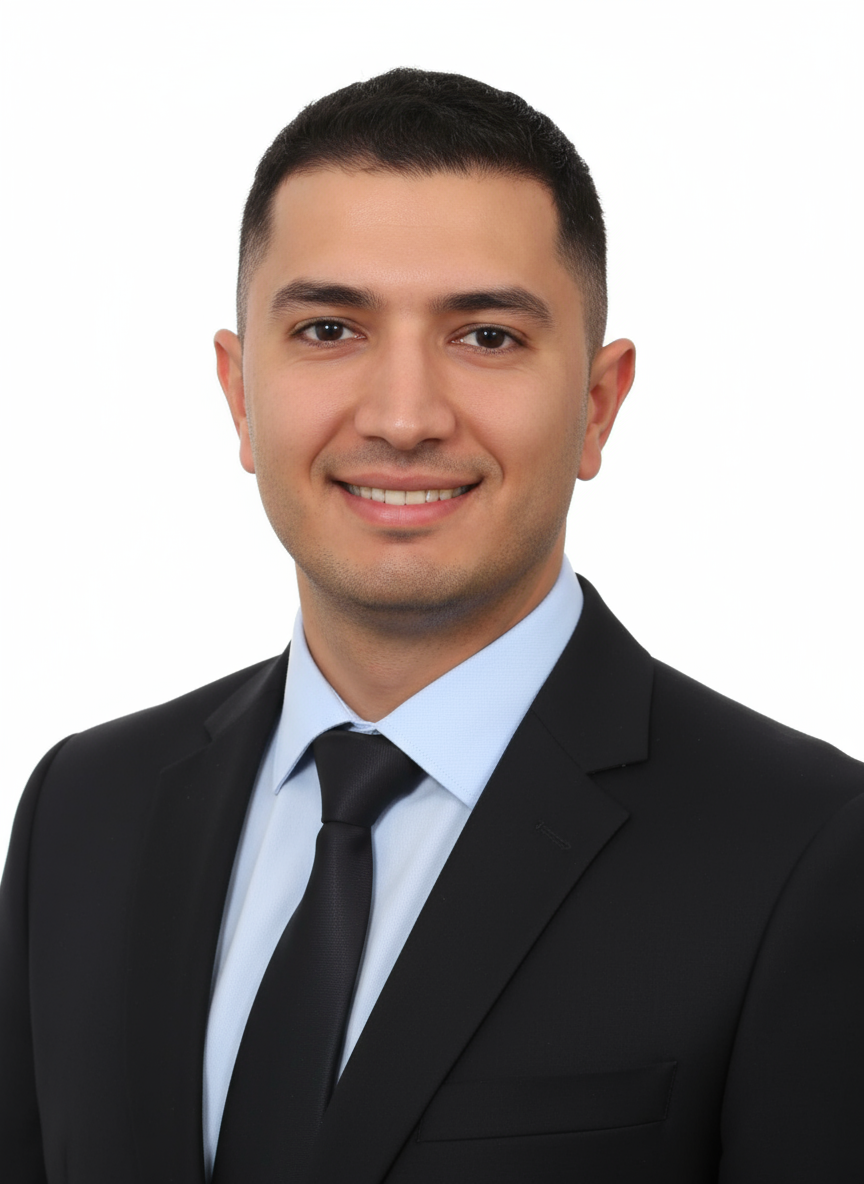
\includegraphics[width=3cm,height=4cm]{presidency photo.png}}
\end{tabularx}

\section*{Profile}
Master’s student in Artificial Intelligence (BTU). Strong software engineering focus with C\#, Python, robust backends, automated testing and releases, cloud, and DevOps. Translates complex technology clearly for both technical and non-technical stakeholders. \textbf{AI-focused software engineer with a strong backend and DevOps foundation.}

\section*{Professional Experience}
\textbf{Software Engineer} \quad Refah Bank, Tehran \hfill 08/2022 to 03/2025\\[-1pt]
\begin{itemize}
  \item Electronic stamp platform on ASP.NET Core (CQRS, MediatR, EF Core, SQL Server); messaging with RabbitMQ/NServiceBus; authentication with IdentityServer; API gateway. \textbf{\(\sim 10{,}000\) requests/day, > 2\,M stamps, MTTR reduced by 40\%}.
  \item Modernized legacy monolith to C\# ASP.NET Core APIs (Clean Architecture, automated tests, Docker, CI/CD). \textbf{Downtime reduced by 30\%}.
  \item Integrated neobank interfaces for \(\sim 200{,}000\) users; improved resilience with retries, circuit breakers, and versioning; enabled team-scale operations.
  \item Architecture and performance tuning across 15+ services and external integrations.
\end{itemize}

\textbf{Software Developer} \quad MAPSA Technology Center, Tehran \hfill 03/2021 to 07/2022\\[-1pt]
\begin{itemize}
  \item Built a WPF/MVVM tool for KPI analysis in oil drilling; optimized asynchronous pipelines; \textbf{reduced reporting time by 40\%}.
  \item Introduced Git workflows and trained teams over 3 months; supported migration from TFS to Git.
\end{itemize}

\textbf{Full Stack Software Engineer} \quad Freelance, Remote \hfill 08/2020 to Present \\[-1pt]
\begin{itemize}
  \item Delivered 12 custom APIs for SaaS/e-commerce; \textbf{p99 latency < 120\,ms}.
  \item Built bots for Telegram, Discord, WhatsApp; significantly reduced manual posting effort.
  \item Implemented CI/CD with Docker and GitHub Actions; cut release times from hours to minutes; zero-downtime deployments.
  \item Migrated 5 SME workloads to Google Cloud with Terraform; \textbf{costs \(\sim 30\%\) lower}; daily cost dashboards.
\end{itemize}

\section*{Projects}
\textbf{Electronic Stamp Platform} \quad Scaling and operations under high load.\\
\textbf{NASA Exoplanet Detection Platform} \quad Led an international 5-person team; end-to-end pipeline for data preparation, modeling, and deployment as Lead Engineer.\\
\textbf{GCP Cloud Resource Analytics} \quad Serverless FastAPI dashboard with Terraform; asset and cost reports.\\
\textbf{Telegram Group Audit Bot} \quad Google App Engine, task queue, lightweight admin interface.\\
\textbf{Social Media Content Automation} \quad Orchestration of platform APIs, scheduling, content generation, and analytics pipelines (automation, monitoring, reporting).\\
\textbf{qrRobust Scanner} \quad Started as a personal project; scaled into an established open-source tool.\\

\section*{Education}
\textbf{Master of Science in Artificial Intelligence} \quad BTU Brandenburg \hfill 03/2025 to Present\\
\textbf{Bachelor of Engineering in Computer Software Engineering} \quad University of Science and Culture \hfill 09/2016 to 10/2020

\section*{Skills}
\begin{multicols}{3}
\begin{itemize}
  \item Programming \& Backend: C\#, Python, SQL, JavaScript/TypeScript, Bash, REST, GraphQL
  \item Frameworks: ASP.NET Core, EF Core, FastAPI, WPF/MVVM
  \item Architecture: Clean Architecture, DDD, CQRS, API Gateway
  \item Data \& Search: SQL Server, PostgreSQL, MySQL, MongoDB, Elasticsearch
  \item Vector Stores: Qdrant, Milvus, Pinecone
  \item Messaging \& Cache: RabbitMQ, Redis
  \item AI/LLM: RAG, LangChain, Transformers, LoRA/QLoRA, prompt design
  \item Data Tools: NumPy, pandas, SciPy, Matplotlib
  \item Cloud \& DevOps: Google Cloud (App Engine, Cloud Run, Cloud Build, Secret Manager), cost dashboards
  \item Automation \& IaC: Docker, Terraform (environments, workspaces, policies)
  \item Orchestration: Kubernetes, Helm
  \item CI/CD: GitHub Actions, Azure DevOps, trunk-based development, release management
  \item Version Control: Git/GitHub, TFS, rebase, squash, cherry-pick, GitFlow
  \item Security \& APIs: IdentityServer, OAuth~2.0, OpenID Connect, JWT, rate limiting, versioning
  \item Testing \& Quality: unit/integration (xUnit, NUnit, pytest), BDD (SpecFlow/Gherkin), Selenium/Playwright, load testing, Jest/RTL
  \item Frontend: HTML, CSS, Bootstrap, Tailwind, React (fundamentals), Redux/Zustand
  \item Build \& Tools: dotnet CLI, pip, poetry, make, nox
  \item Product \& Delivery: MVP scoping, requirements analysis, SRS/BRD, backlog grooming, Scrum/Kanban, code review, documentation
  \item Collaboration: Azure Boards, Jira, Figma, Visio, UML
  \item Research \& Writing: LaTeX/Overleaf, literature review, bibliometric studies
\end{itemize}
\end{multicols}

\section*{Publications}
\begin{itemize}
  \item A Bibliometric Analysis of Quantum Machine Learning Research. \emph{Journal of Science and Technology Libraries}, 2024. \href{https://doi.org/10.1080/0194262X.2023.2292049}{DOI}
  \item Text Independent Speaker Recognition — A Novel Deep Learning Approach. \emph{CoDIT}, 2024. \href{https://doi.org/10.1109/CoDIT62066.2024.10708578}{DOI}
  \item Cost Efficiency in Cloud Data Centers via Model Free Q Learning. \emph{ICEEE}, 2024. \href{https://doi.org/10.1007/978-981-97-9112-5_27}{DOI}
\end{itemize}

\section*{Certifications}
\begin{itemize}
  \item Docker Foundations Professional Certificate — Docker Inc — 2024
  \item ASP.NET for Experienced Developers Specialization — Coursera and Brood Infinity — 2024
  \item Career Essentials in Generative AI — Microsoft
  \item Microservice and Deployment — Coursera
  \item Programming in C\# Certification — Technical Institute of Tehran — first in cohort
  \item AI Ethics — LinkedIn Learning
\end{itemize}

\section*{Languages}
Persian (native) \quad English (C1) \quad German (A2)

\section*{Availability}
Based in Cottbus; flexible part-time during the semester; increased hours during semester breaks; remote and on-site by arrangement.

\section*{Links}
GitHub Portfolio  \href{https://github.com/ArmanShirzad}{github.com/ArmanShirzad}\\
LinkedIn  \href{https://linkedin.com/in/arman-shirzad}{linkedin.com/in/arman-shirzad}\\
Personal Website  \href{https://armanshirzad.guru}{armanshirzad.guru}

\end{document}
